\section{Preliminary Experiments}
\label{sec:experiment}
In this section, we did the experiments by comparing applying a model
checker to original C language programs with to abstracted
behavior. Figure~\ref{fig:statistic} shows the results of the
experiments. All of the experiments are done on a machine with an
Inter(R) Core i5-4590 3.30Hz CPU, 6MB cache and 8GB memory, running
Debian (kernel version) and CPAchecker (version 1.3.2).

In Figure~\ref{fig:statistic}, the meaning of each column is described
as follows. There are mainly two columns, \texttt{original programs}
and \texttt{abstracted behavior}, which means applying the model
checker to a original C language program and to abstracted behavior
respectively. These two columns consist of several columns:
$\sharp$\texttt{loc} means the number of program locations;
$\sharp$\texttt{fun} means the number of functions in a program;
\texttt{cpu time (total)} means the total execution time of CPU in
seconds; \texttt{memory(MB)} means the number of virtual memory cells
consumed by model checker in \texttt{MByte}; \texttt{fixed num} means
the number of available memory cells which we fix; the \texttt{true}
or \texttt{false} behind \texttt{fixed num} means it is \texttt{true}
if the number of the memory cells which a program consumes does not
exceed the \texttt{fixed num}, otherwise it is \texttt{false}.

The programs used for the experiments are described as follows:
\begin{itemize}
\item \texttt{linklist.c} and \texttt{linklist2.c} initialize a list,
  and perform some operations on the list (insert , delete, locate a
  node and traverses the list), and destroy the list. The difference
  between \texttt{linklist.c} and \texttt{linklist2.c} is that the
  former creates list by the head-insertion, whereas the latter creates a list
  by the tail-insertion.
\item \texttt{linkstack.c} creates a stack, pushes some elements in
  the stack, traverses the stack and clear the stack.
\item \texttt{linkqueue.c} initializes a queue, inserts, deletes some
  elements in the queue, clears the queue and destroys the queue.
\item \texttt{binarysorttree.c} inserts some nodes in a binary tree
  and deletes all the allocated nodes.
\item \texttt{database.c} models a database. It opens a database and
  performs some operations on the database (retrieve, delete and
  update data, or create a new database) and closes the database.
\item \texttt{ihex2fw.c} is a file from Linux kernel
  \texttt{/firmware/ihex2fw.c}, which converts ihex files into binary
  representation for use by Linux kernel.
\item \texttt{gen\_init\_cpio.c} is a file from Linux kernel
  \texttt{/usr/gen\_init\_cpio.c}, which produces a binary file which
  performs on a file containing newline separated entries that
  describe the files to be included in the initramfs archive.
\end{itemize}

The results present in the Figure~\ref{fig:statistic} show that the
resources required for model checking become smaller if applying model
checkers to the abstracted behavior, since the abstracted behavior
only consists of allocation and deallocation.

One thing we should notice in Figure~\ref{fig:statistic} is that for
each line, the result of \texttt{true} or \texttt{fals}e in
the\texttt{fixe num} column should be the same when model checking on
original programs and abstracted behavior, but it is not, for example,
\texttt{linklist.c} has the \texttt{true} under \texttt{original
  programs} column but the false under \texttt{abstracted behavior}
column. The reason is that our approach, abstracted behavior, can not
deal with conditional statements, function calls in another files,
loop statements, for example, the \texttt{linklist.c} consists of
statements like if-then-else and for-loop statements, which is
abstracted as $\Malloc;\mu\alpha.((\Malloc;\alpha) +
0));\mu\alpha.((\Free;\alpha) + 0)$. In fact, the \texttt{linklist.c}
does $\Malloc$ 6 times, and then $\Free$ 6 times, so it is safe; but
the abstracted behavior may perform like
$\Malloc;\mu\alpha.(\Malloc;\alpha));0$, this means consuming unbound
number of memory cells.

\begin{table}
\begin{tabular}{|c|c|c|c|c|c|}
\hline
& \multicolumn{5}{|c|}{original programs}  \\
\hline
 & $\sharp$loc & $\sharp$fun & cpu time (total) & memory (MB) & fixed num \\
\hline
linklist.c & 154 & 13 & 9.770 & 2943 & 6(true)  \\
\hline
linklst2.c & 140 & 13 & 25.620 & 2955 & 21(true) \\
\hline
linkstack.c  & 87 & 10 & 10.830 & 2941 & 11(true) \\
\hline
linkqueue.c & 119 & 11 & 13.110 & 2939 & 4(true) \\
\hline
binarysorttree.c & 80 & 5 & 30.210 & 2950 & 10(true)  \\
\hline
database.c & 179 & 12 & 4.930 & 2922 & 3(true) \\
\hline
ihex2fw.c & 202 & 7 & 23.490 & 2882 & 5(false) \\
\hline
gen\_init\_cpio.c & 346 & 19 & 9.580 & 2809 & 1(true) \\
\hline
\end{tabular}
%%\caption{My first table}
\end{table}

\begin{table}
\begin{tabular}{|c|c|c|c|c|c|}
\hline
&\multicolumn{5}{|c|}{abstracted behavior} \\
\hline
 &$\sharp$loc & $\sharp$fun & cpu time (total) & memory (MB) & fixed num \\
\hline
linklist.c &  20 & 4 & 3.190 & 2918 & 6(false) \\
\hline
linklst2.c & 20 & 4 & 10.72 & 2945 & 21(false) \\
\hline
linkstack.c & 20 & 4 & 4.990 & 2916 & 11(false) \\
\hline
linkqueue.c & 25 & 4 & 2.660 & 2919 & 4(false) \\
\hline
binarysorttree.c & 19 & 4 & 5.130 & 2935 & 10(false) \\
\hline
database.c  & 21 & 4 & 2.760 & 2920 & 2(false) \\
\hline
ihex2fw.c  & 15 & 4 & 2.160 & 2797 & 5(false) \\
\hline
gen\_init\_cpio.c & 15 & 4 & 2.160 & 2799 & 1(false) \\
\hline
\end{tabular}
%%\caption{My first table}
\end{table}


%% \begin{table}
%% \tiny
%% \begin{tabular}{|c|c|c|c|c|c|c|c|c|c|c|}
%% \hline
%% & \multicolumn{5}{|c|}{original programs} & \multicolumn{5}{|c|}{abstracted behavior} \\
%% \hline
%%  & $\sharp$loc & $\sharp$fun & cpu time (total) & memory (MB) & fixed num & $\sharp$loc & $\sharp$fun & cpu time (total) & memory (MB) & fixed num \\
%% \hline
%% linklist.c & 154 & 13 & 9.770 & 2943 & 6(true) & 20 & 4 & 3.190 & 2918 & 6(false) \\
%% \hline
%% linklst2.c & 140 & 13 & 25.620 & 2955 & 21(true) & 20 & 4 & 10.72 & 2945 & 21(false) \\
%% \hline
%% linkstack.c  & 87 & 10 & 10.830 & 2941 & 11(true) & 20 & 4 & 4.990 & 2916 & 11(false) \\
%% \hline
%% linkqueue.c & 119 & 11 & 13.110 & 2939 & 4(true) & 25 & 4 & 2.660 & 2919 & 4(false) \\
%% \hline
%% binarysorttree.c & 80 & 5 & 30.210 & 2950 & 10(true) & 19 & 4 & 5.130 & 2935 & 10(false) \\
%% \hline
%% database.c & 179 & 12 & 4.930 & 2922 & 3(true) & 21 & 4 & 2.760 & 2920 & 2(false) \\
%% \hline
%% ihex2fw.c & 202 & 7 & 23.490 & 2882 & 5(false) & 15 & 4 & 2.160 & 2797 & 5(false) \\
%% \hline
%% gen\_init\_cpio.c & 346 & 19 & 9.580 & 2809 & 1(true) & 15 & 4 & 2.160 & 2799 & 1(false) \\
%% \hline
%% \end{tabular}
%% %%\caption{My first table}
%% \end{table}

%% \begin{figure}
%%  \centering
%%  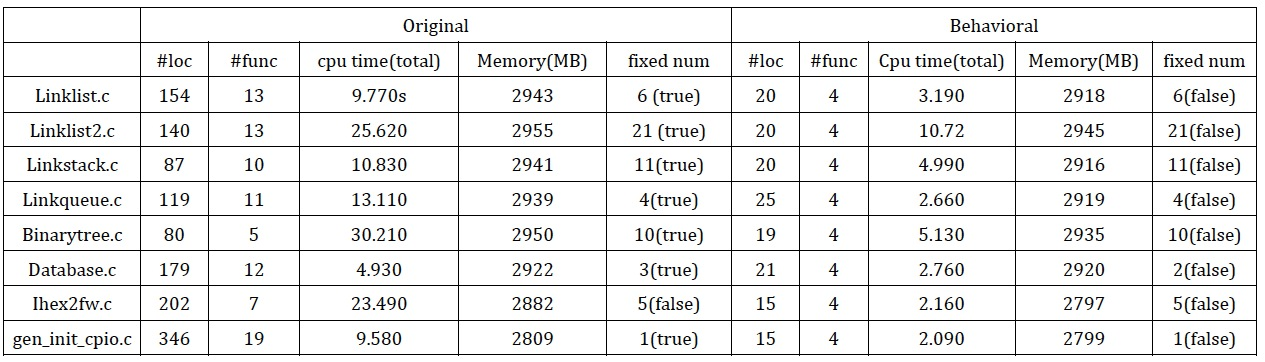
\includegraphics[width=14cm]{statistic.png}
%% \caption{Comparison}
%% \label{fig:statistic}
%% \end{figure}
